\documentclass{article}
\usepackage{listings}
\usepackage{tabto}
\usepackage{graphicx}
\usepackage{amssymb}
\lstset{breaklines=true, language=c++}
\usepackage[margin=0.75in]{geometry}
\begin{document}
\begin{center}
\textbf{\LARGE ECE 49600 Optimizing Point Cloud Algorithm}
\end{center}
~\\
Project title: \tab GPU Processing of kNN Query Points in Groups\\
Name of student: \tab Yi En Gan (Andrew)\\
Name of instructor: \tab Milind Kulkarni\\
Term: \tab Spring 2020\\
Credit hours: \tab 2\\
\\
\large
\noindent
\textbf{INTRODUCTION}\\
\normalsize
\newline
A naive kNN algorithm compares each query with all other data points in $O(n^{2} log(k))$. Both the solving of a kNN problem and verification of a kNN solution consume very large amount of time with respect to the data size.\\
\\
Instead of performing naive kNN, an approximate kNN was used. A hybrid tree structure represents data points in kd-space with each node in the tree representing a range in kd-space. The root node represents the entire space and initially contains all data points. The space is then partitioned into two subspaces and the data points are inherited by the two child nodes. A hybrid tree allows the boundaries of the subspaces to overlap depending on $\rho$ and the number of data points inherited by each child node. The partitioning repeats until the child node has either one or no data point. If only spill nodes are created, the runtime of kd-tree kNN will be $O(n$ $log(n)$ $log(k))$.
\begin{center}
 \begin{tabular}{||c c c c||} 
 \hline
 Node & Condition for creation & Characteristics & Traversal\\ [0.5ex] 
 \hline\hline
 Spill & numpoint(left or right) $\leq$ $\rho$ numpoint(parent) & boundaries overlap & DFS with no backtracking \\ 
 \hline
 Metric & numpoint(left or right) $>$ $\rho$ numpoint(parent) & boundaries do not overlap & backtracking required\\
 \hline
\end{tabular}
\end{center}
~\\
The GPU allows for efficient parallelism of simple yet repetitive tasks. In this project, Nvidia's CUDA framework was used to run algorithms on the GPU and the kNN algorithm was used to observe how an algorithm can be optimized for the GPU. Methods incorporated into this project include autoroping, lockstep traversal and hybrid tree[1].\\\\
\large\noindent
\textbf{RESULTS}\\
\normalsize
\newline
\textbf{i. Execution on CPU:}\\
Four types of kNN algorithms were implemented. They were naive kNN, recursion kNN, autoroping kNN and parallel kNN. All but the first kNN utilized the hybrid tree structure. Overlapping subspaces account for data points near the partition border[2]. It was found that for a uniformly random distribution of data points, the number of nodes visited was minimum at $\rho$ = 0.75 to 0.8.\\
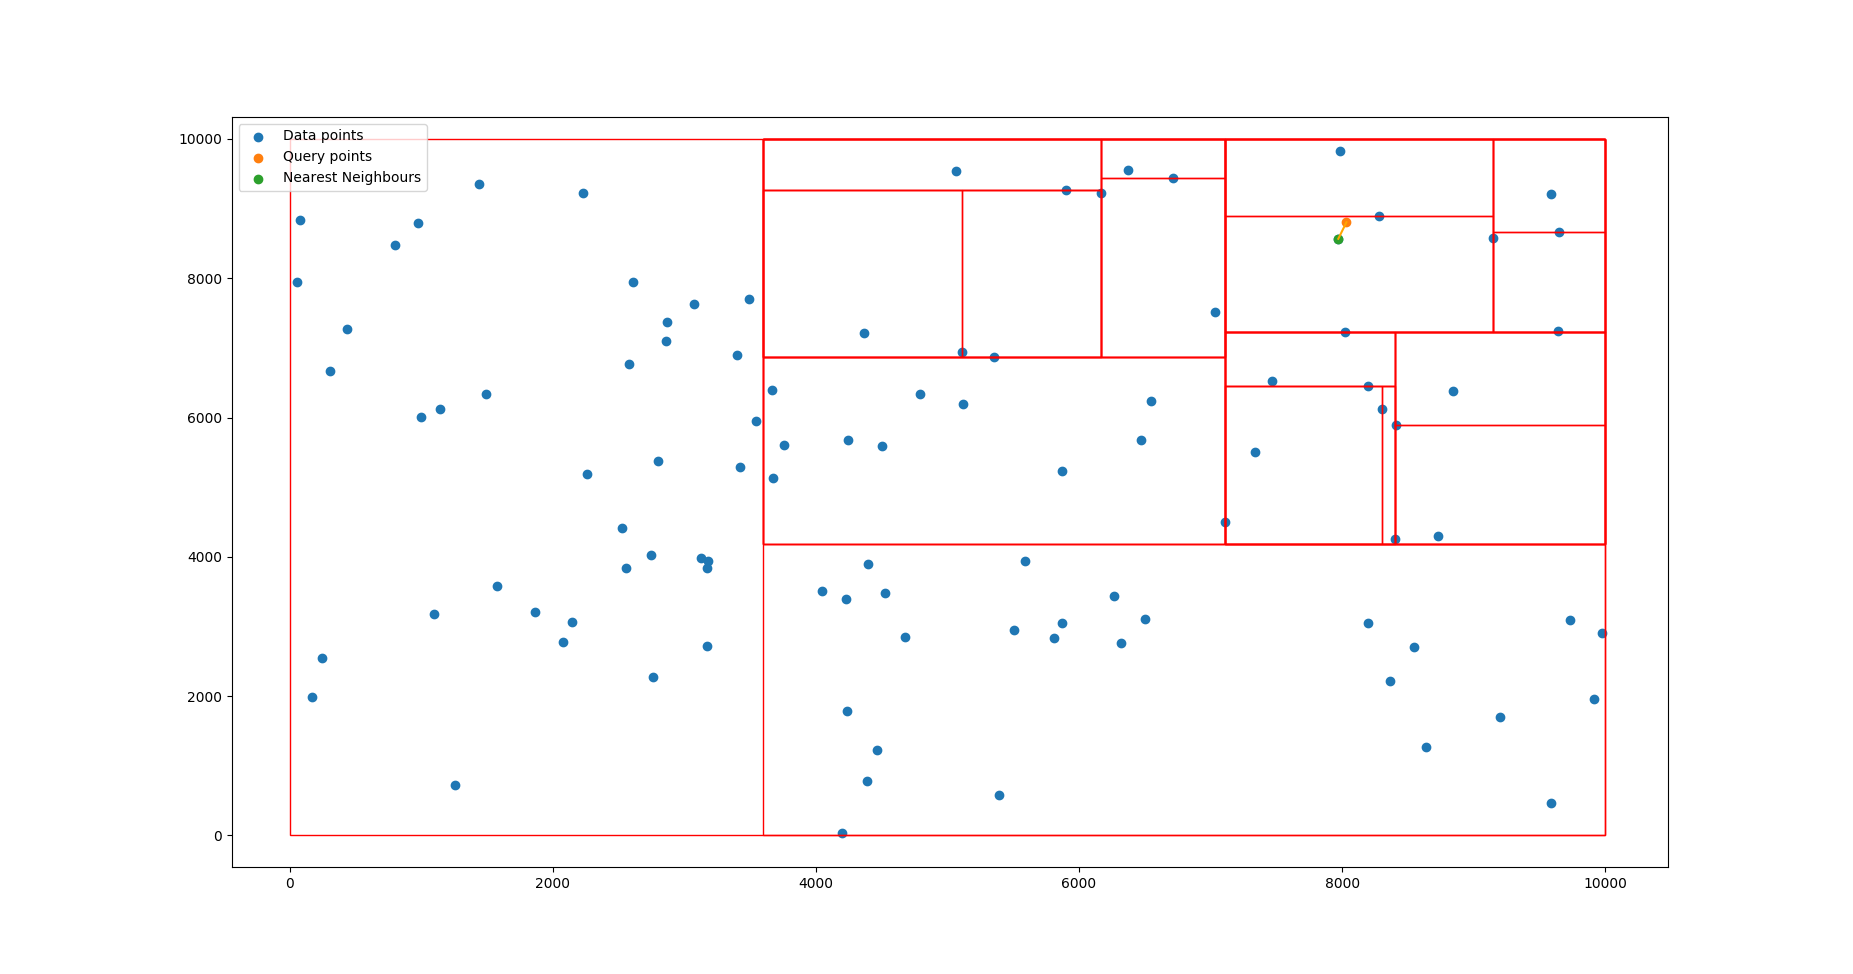
\includegraphics[scale=0.36]{../sptree/visualization/chart_points_partition}
\newpage\noindent
The cost of finding the nearest point of a query was at its peak at $\rho$ = 0 to 0.5\\
The proportion of spill nodes in the tree increases with $\rho$. As $\rho$ $>$ 0.8, the cost rises again. At this point, the presence of data points in the overlapping region were duplicated in both child nodes, causing the spill nodes to keep dividing until a node contains only one or no points. This greatly increases the height of the tree. A balance in $\rho$ is needed to achieve balance between accuracy and efficiency.\\
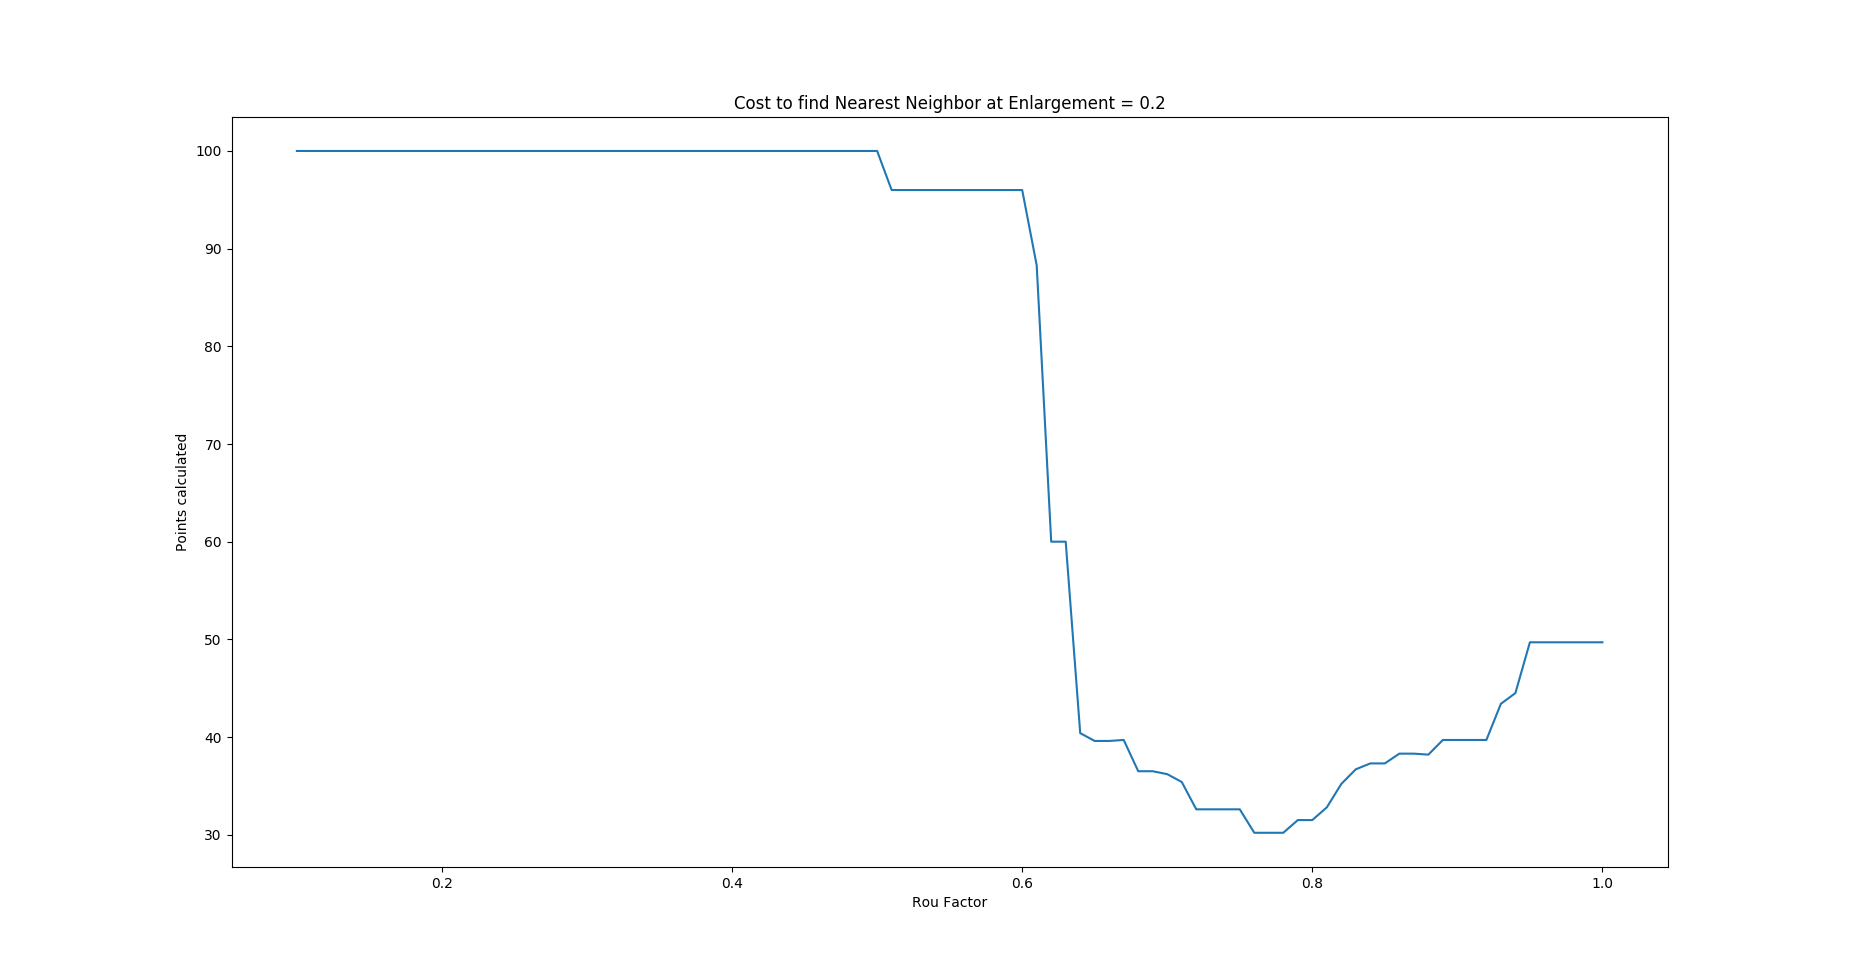
\includegraphics[scale=0.38]{../sptree/visualization/chart_cost_rou}
\\\\
The accuracy of the results largely correspond with the cost of search. Regardless of $\rho$, the accuracy remains above 98\%. the nodes were being expanded by a factor of 0.2.\\
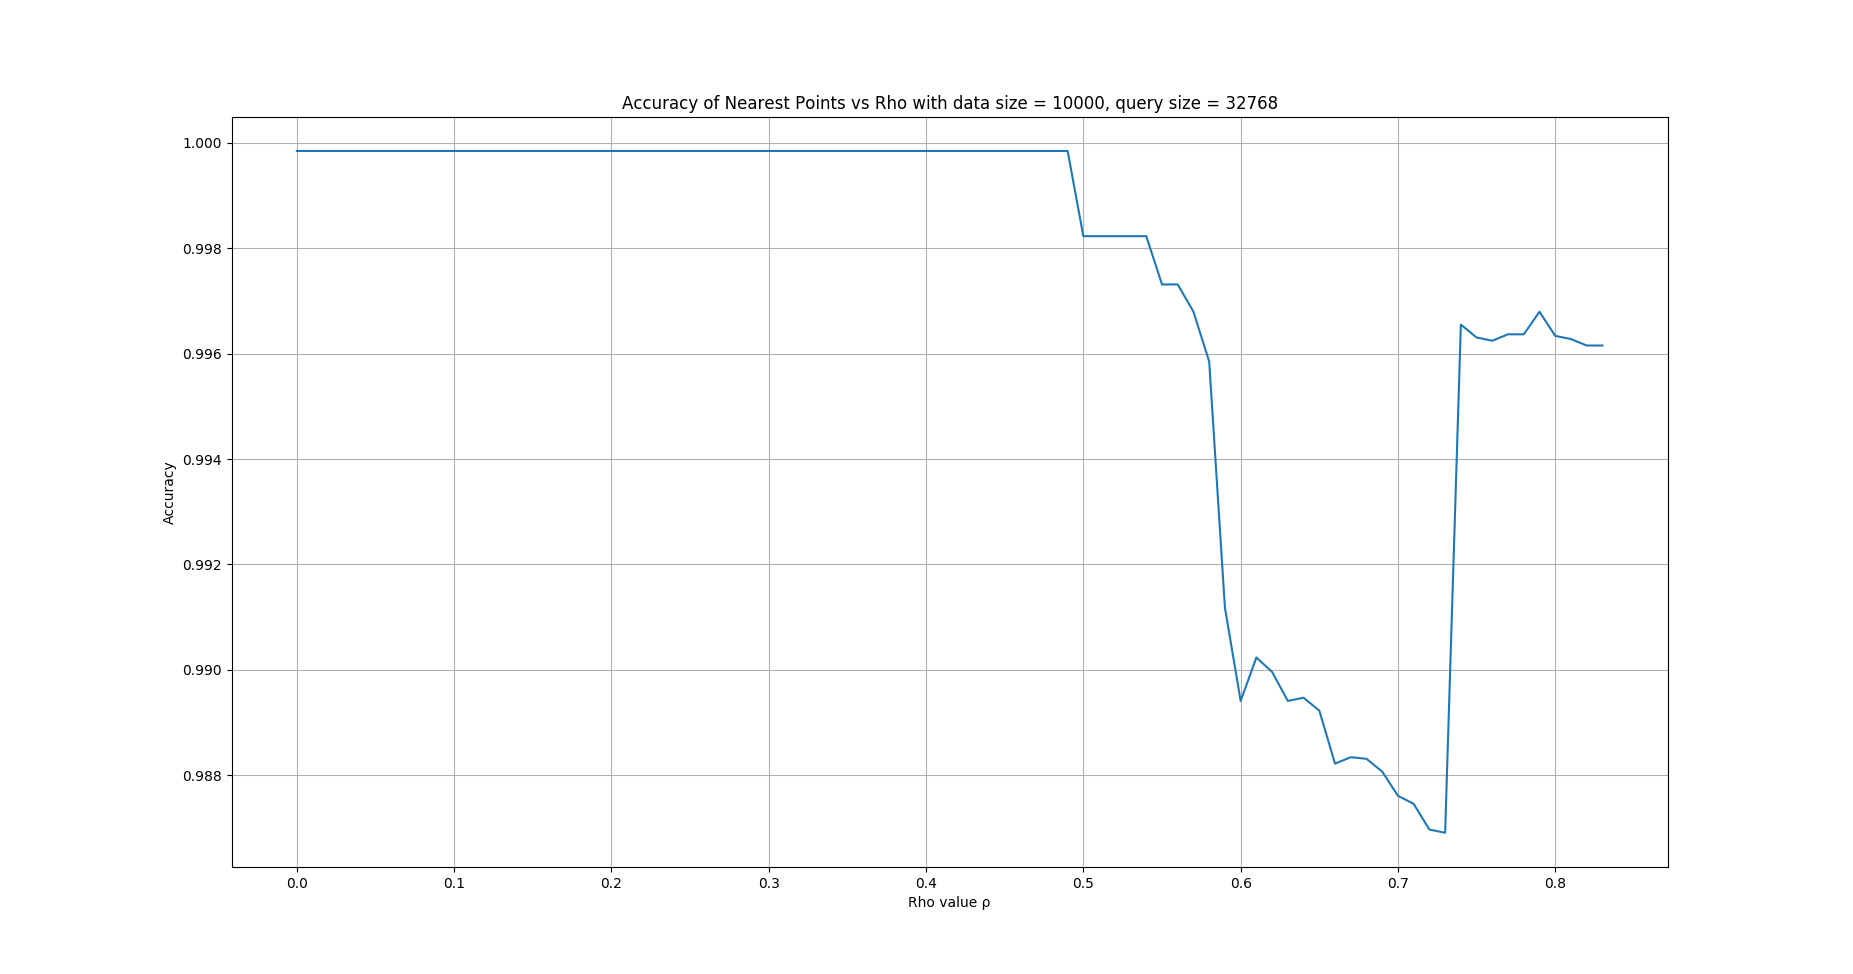
\includegraphics[scale=0.38]{../sptree/visualization/chart_accu_rou}
~\\
Finally, a kNN algorithm running on parallel using Intel's TBB library was implemented to simulate the algorithm in a multithreading environment. It was noted that the runtime remained more consistent as the query size increased.\\
\newpage\noindent
\textbf{ii. Execution on GPU}\\
Autoroping is a process of transforming a recursive call into an iterative process. The effect of autoroping on CPU runtime was minimal due to the negligible overhead of popping the return address out of the stackframe. However, autoroping is very crucial for GPU execution. A GPU has less memory allocated for storing return addresses. As a result, the CUDA architecture has a recursion depth limit of 24 as of Compute Capability 3.5 [4], which made it difficult for traversing any kind of tree structure that grows in relation to the data size.\\
\small
\begin{lstlisting}
void kNN_autorope(Node* root, Point query):
    nodeStack.push(root);
    
    while(!nodeStack.isEmpty()):
        Node* root = nodeStack.pop();
        
       	if(root->nodeType == METRIC_NODE):
            nodeStack.push(root->right);
            nodeStack.push(root->left);
            
        else if (root->nodeType == SPILL_NODE):
            if(root->right->inside(query)) nodeStack.push(root->right);
            if(root->left->inside(query)) nodeStack.push(root->left);
\end{lstlisting}
\normalsize
~\\
The workload was divided among the threads by allowing the threads to access query points stored in contiguous memory in a global array to achieve memory coalescing, i.e. efficient memory transaction by accessing coontiguous memory locations [3].\\
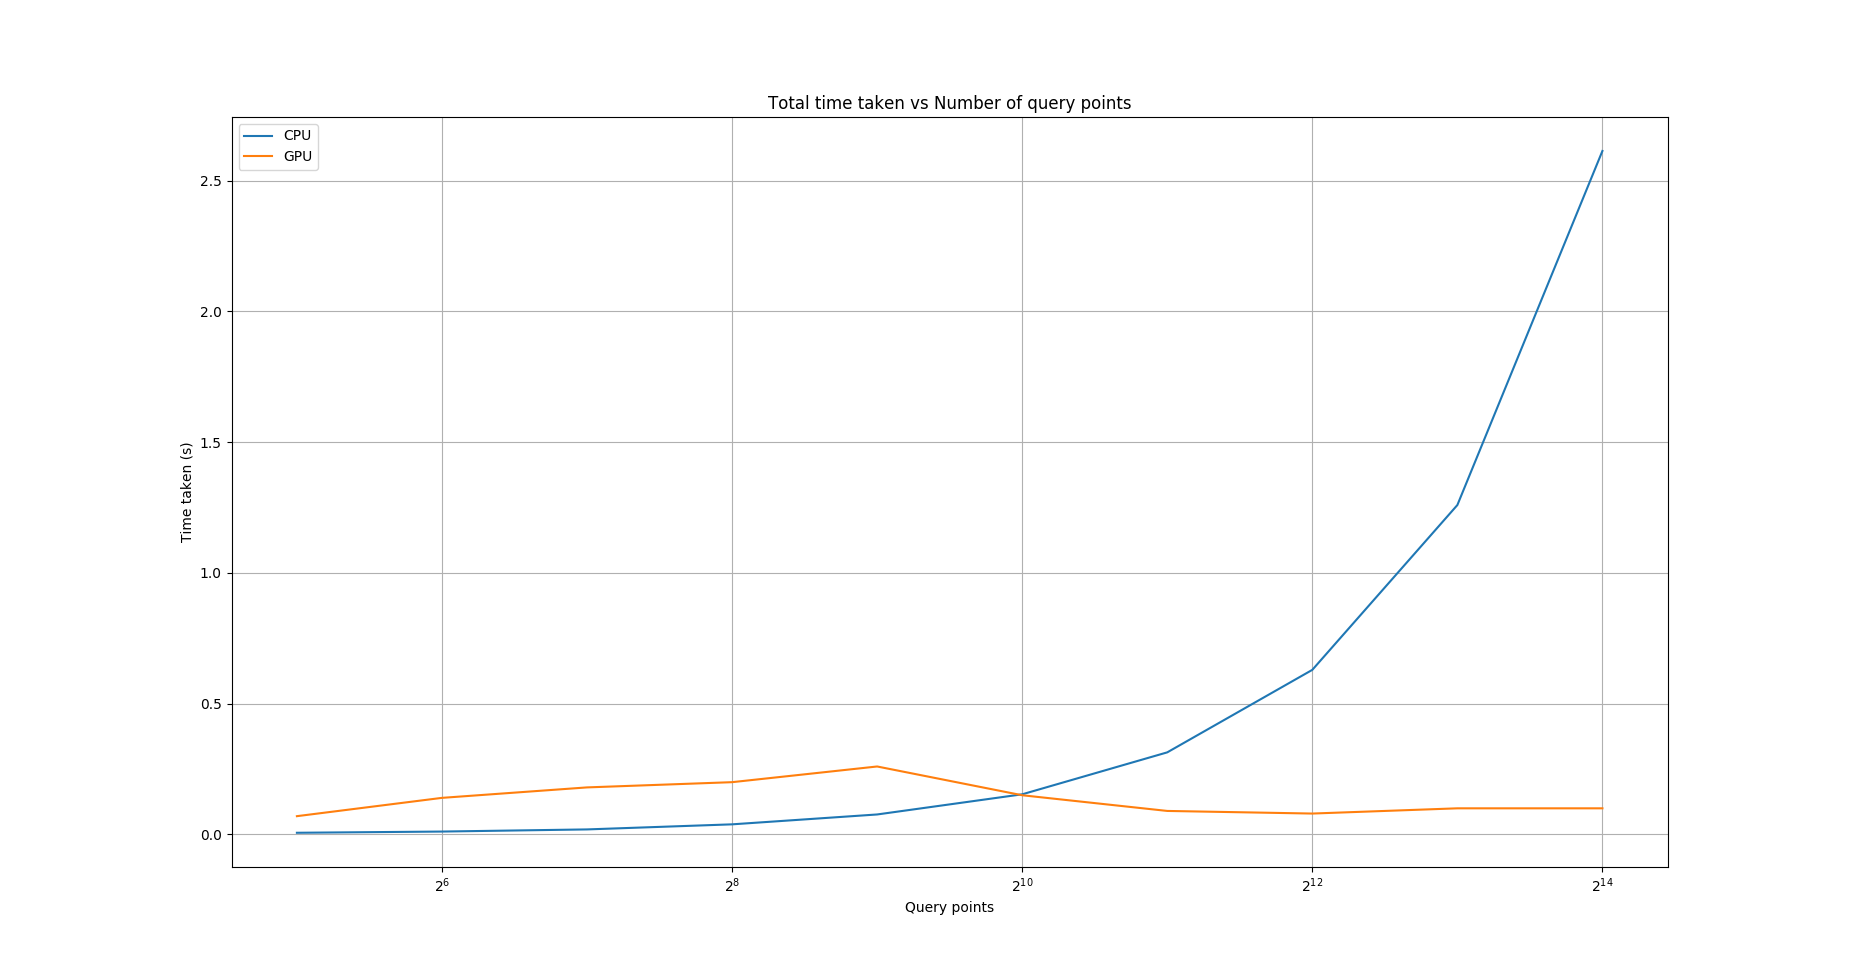
\includegraphics[scale=0.38]{../batchtree/graphs/cpu_gpu_total}
\\
With the data size fixed, the number of query points provided was increased exponentially. It was noted that while the runtime on CPU increased exponentially as expected, the runtime on GPU was fairly consistent except for a spike at number of query = 512\\
\\
This was due to each block consisting of 512 threads for the purpose of the project. The spike occurs at the number of threads created per block. When the number of query was below the number of threads per block, only one block was allocated and partially used. This causes the remaining threads to not be in use, resulting in wastage. Furthermore, the low number of threads means that the overhead of allocating a block, spawning the threads, and deallocating the block exceeds the reward of parallelism.\\
\newpage\noindent
\textbf{iii. Improved execution on GPU}\\
Query points that are nearby may end up traversing the same path in the first few layers of the tree. This becomes more apparent when the query points are more densely located rather than uniformly distributed. Traversal of nearby nodes along the same path multiple times can be viewed as a redundancy. There must be a way to exploit the locality of query points that are close together so that repeated paths can be explored in one iteration.\\
\\
\begin{center}
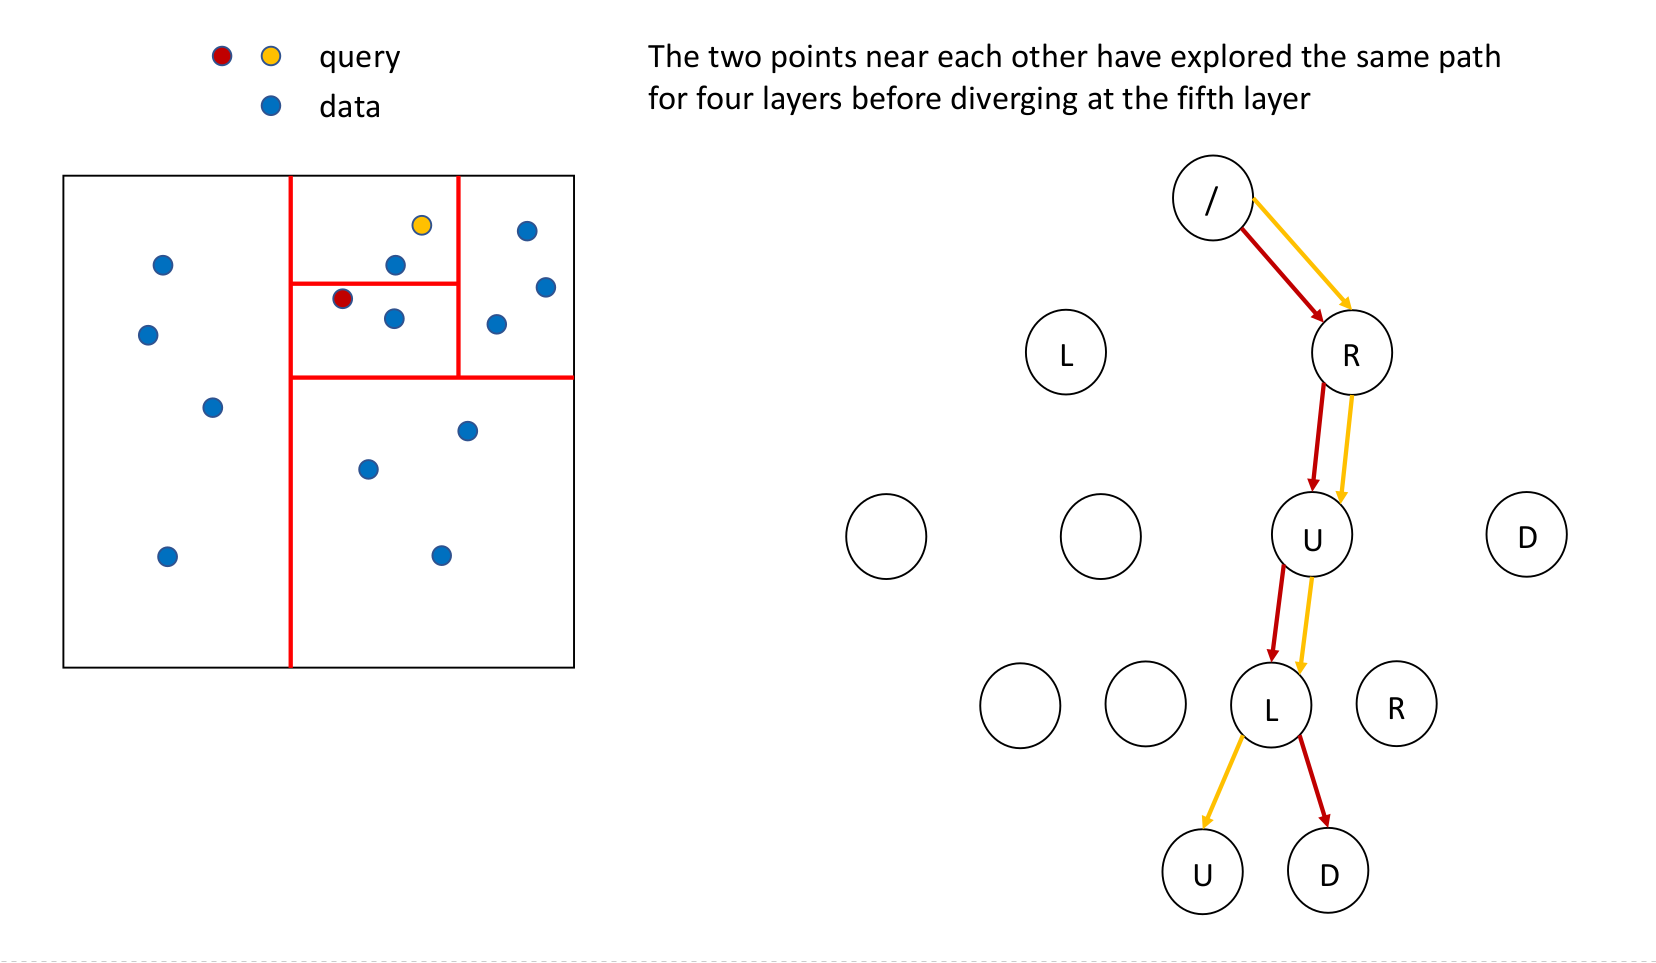
\includegraphics[scale=0.25]{00}
\end{center}
A method to reduce the redundancy was to process query points in groups based on locality.\\
When a list of query points were received, the query points were partitioned and placed in groups based on locality. For the purpose of the project, the query points were assumed to be uniformly randomly distributed, and so the grouping of query points solely depend on their absolute positions in the kD space.\\
\begin{center}
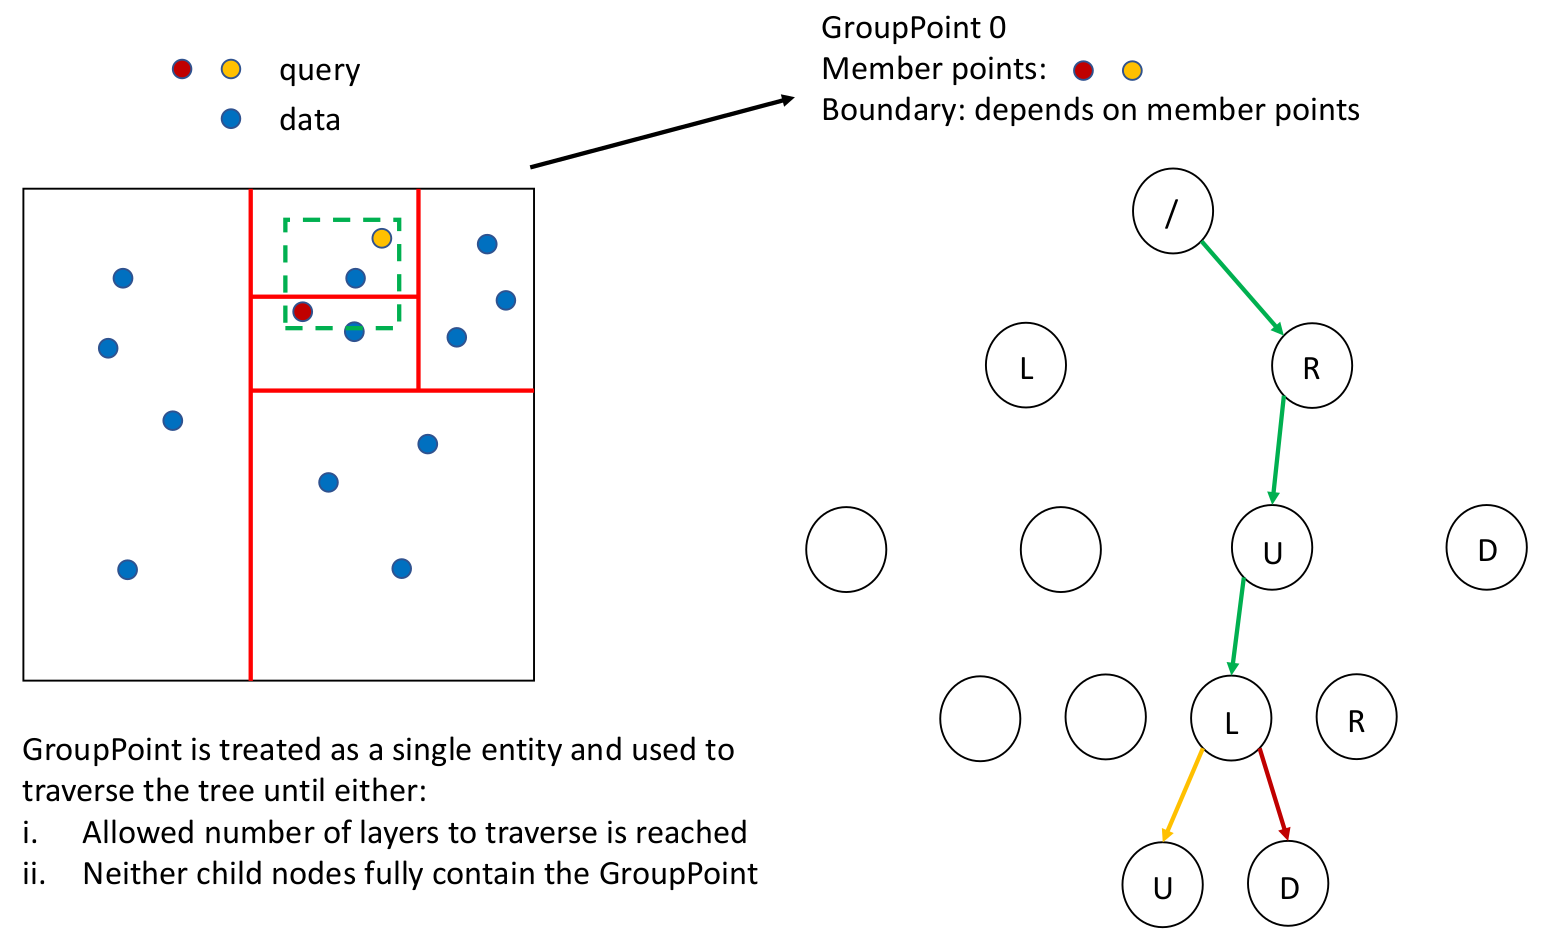
\includegraphics[scale=0.25]{01}
\end{center}
\newpage\noindent
\textbf{iv. Implementation}\\
Every GroupPoint traversed the tree on the CPU side until the node
where the GroupPoint must disperse its member queries was reached.
All query points belonging to the same group should have the same ‘continueNode’, the node at which the GroupPoint traversal ended.\\
\\
The queries, along with their ‘continueNode’ were now cast into a flat
array and handed over to the GPU. Instead of always starting the traversal at node 0 (root node), the device function allows the traversal to begin at the corresponding ‘continueNode’ of the query being processed.\\
\\
\large
\textbf{EXPLANATION}\\
\normalsize
\newline
The graph below shows the improvement in performance when query points were processed in groups (or batches). The maximum number of nodes allowed for the group to traverse was fixed at 3.\\
\\
Time taken to process query points using CPU (blue), GPU (orange) and improved GPU (green).\\
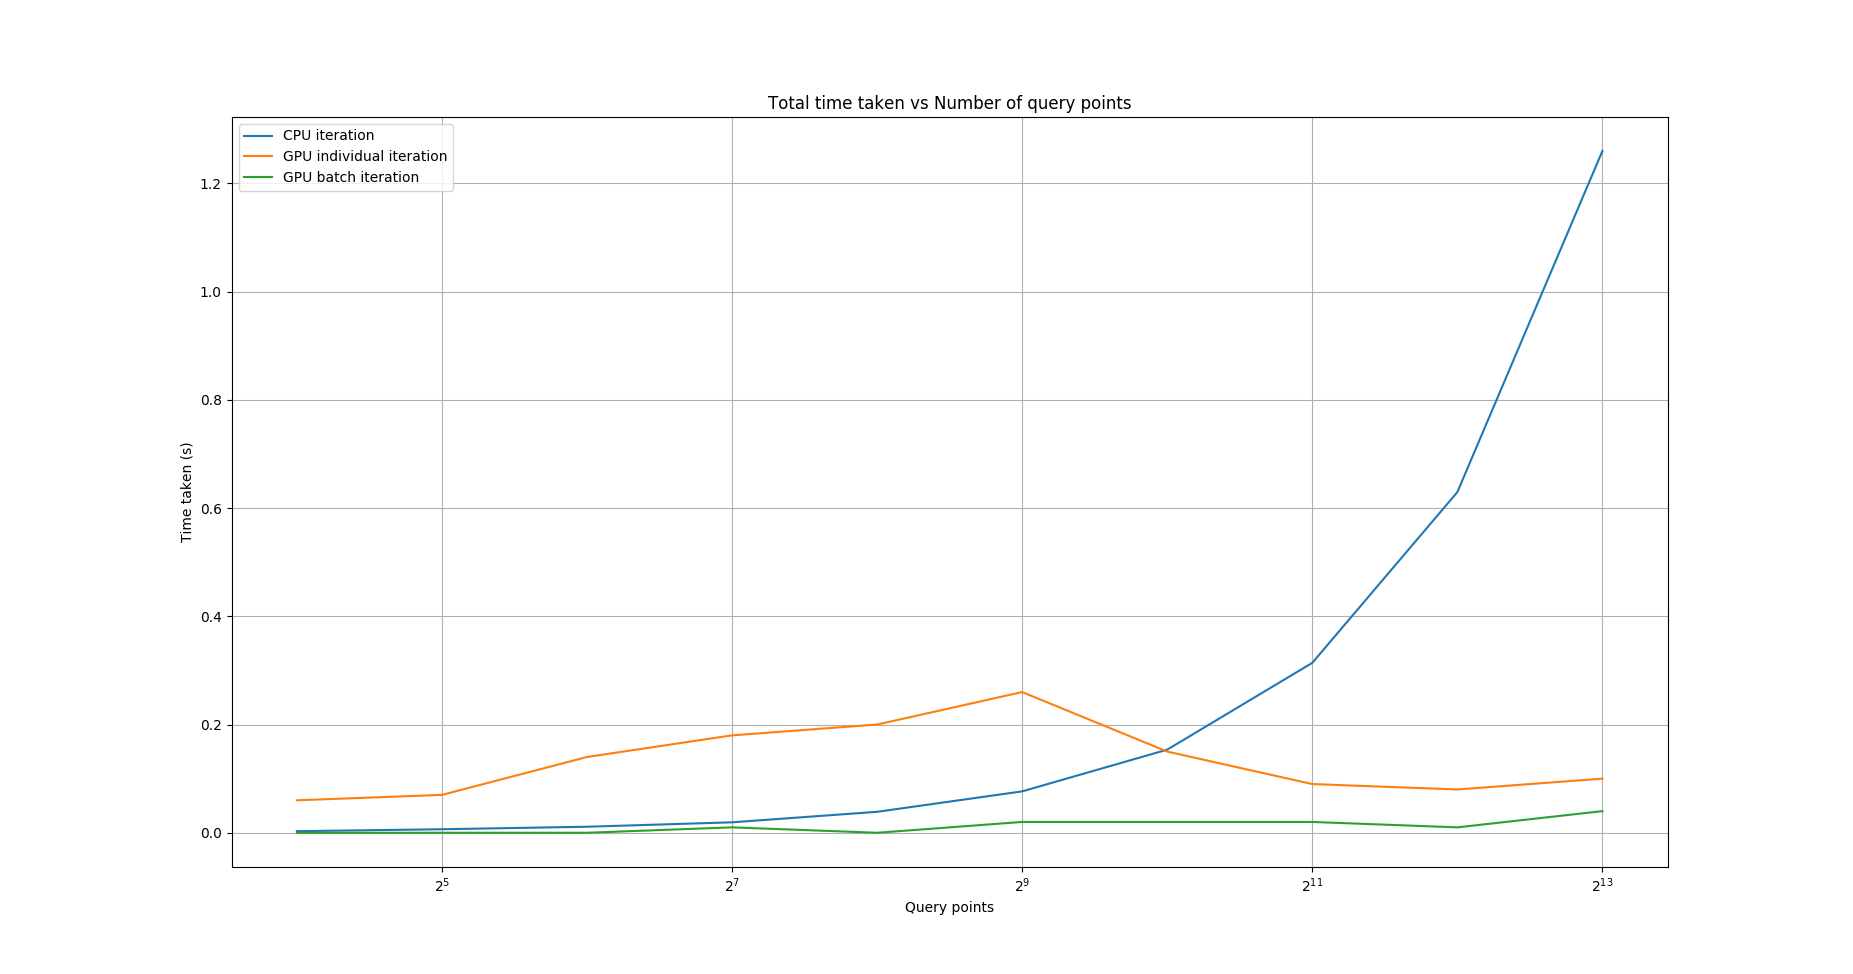
\includegraphics[scale=0.38]{../batchtree/graphs/cpu_gpu_batch}\\
Time taken vs max layers to traverse in group (left) and accuracy vs max layers to traverse in group (right)\\
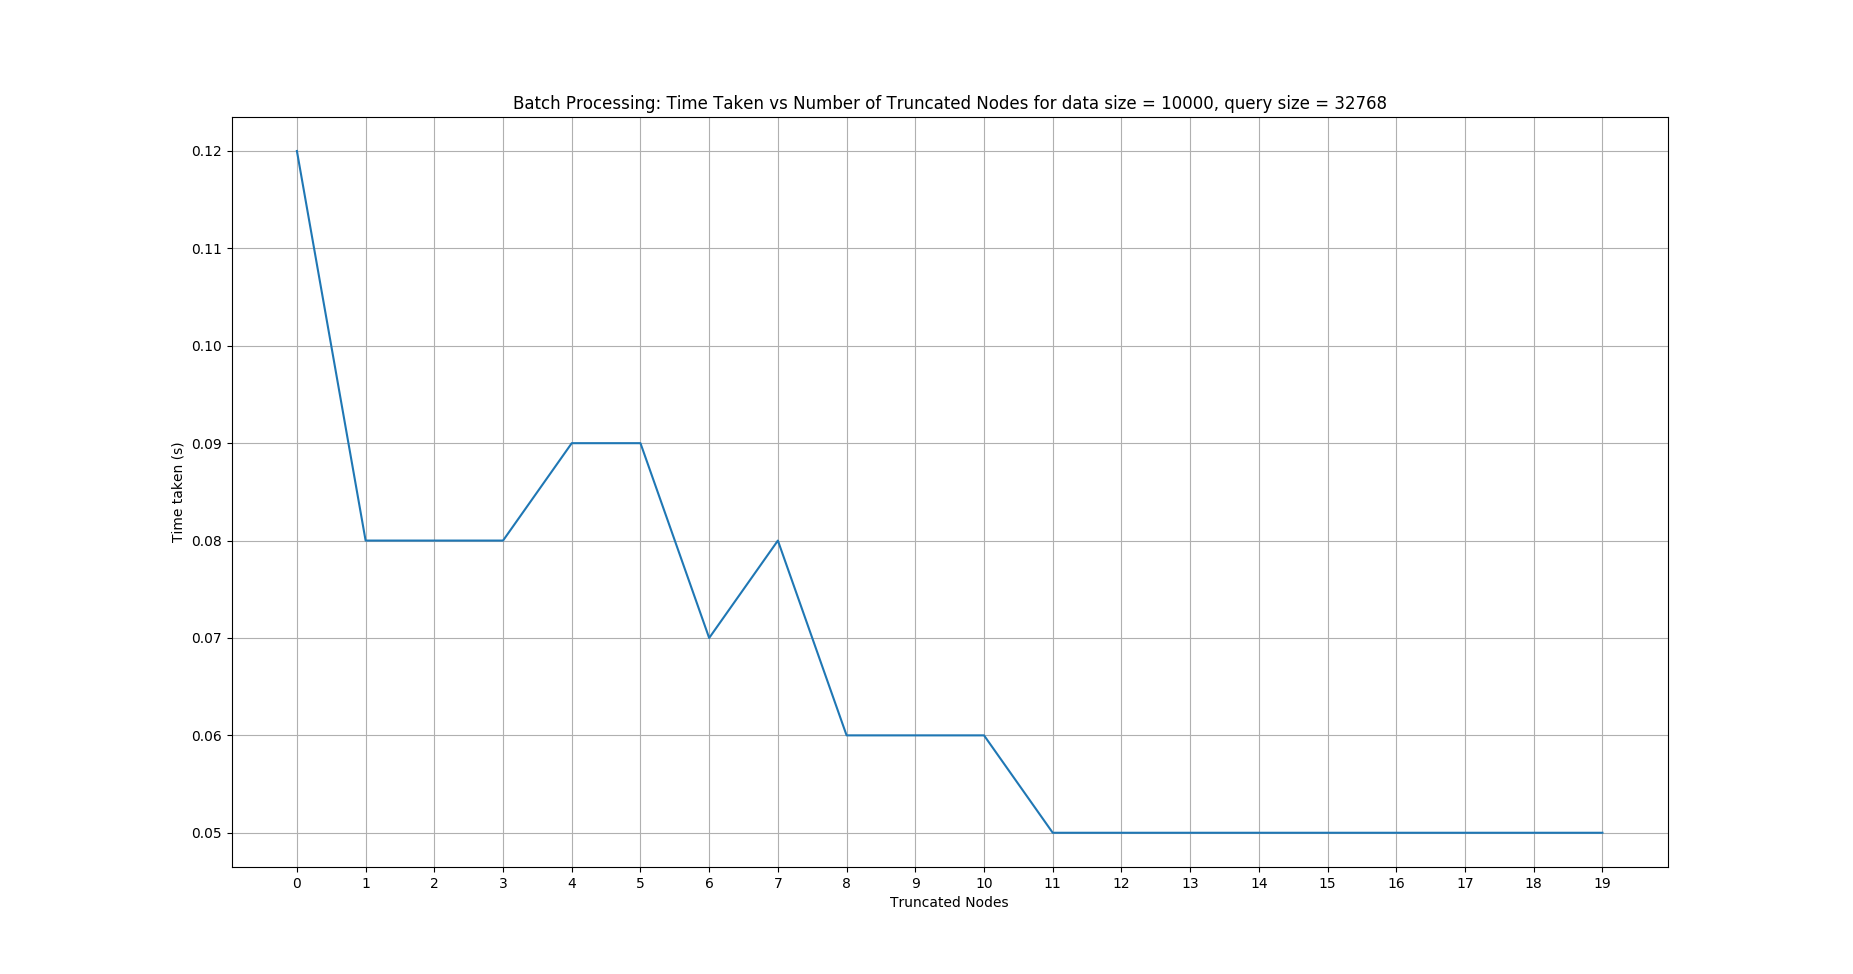
\includegraphics[scale=0.18]{../batchtree/graphs/batch_time}
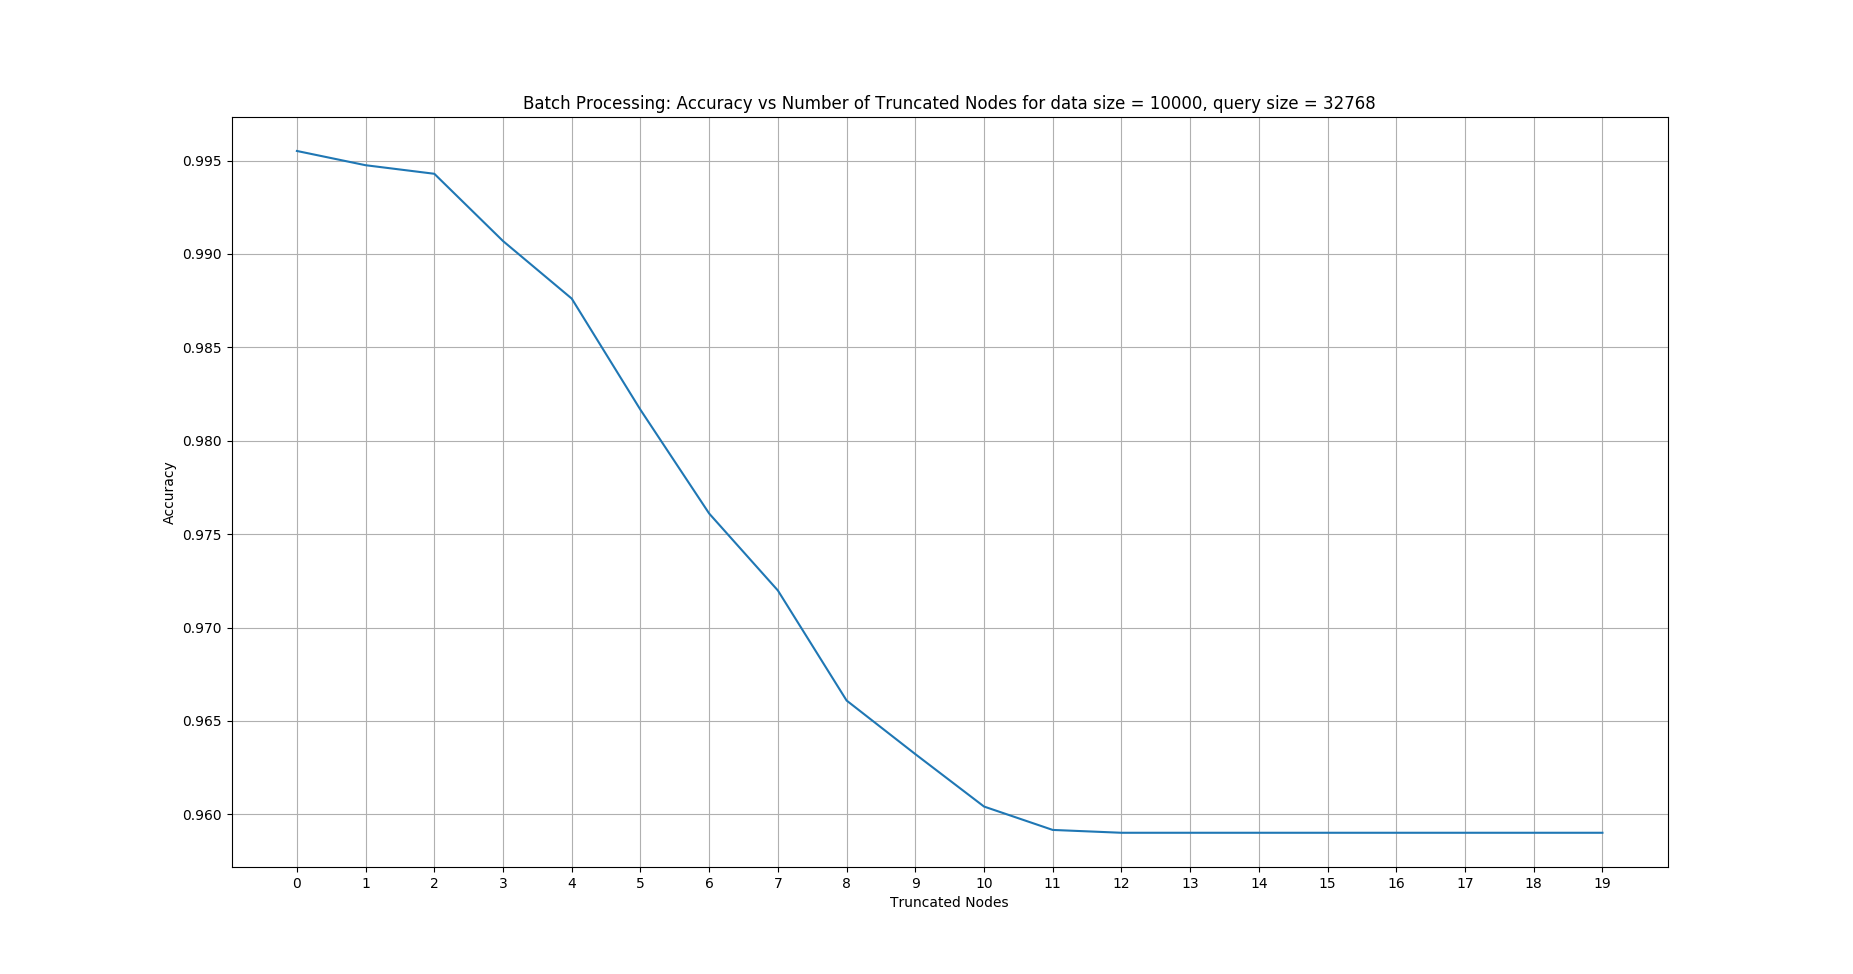
\includegraphics[scale=0.18]{../batchtree/graphs/batch_accu}\\
\\
By processing the query points in groups, the redundancy of exploring the same path by nearby query points was significantly reduced. However, the approximation did result in a decrease in accuracy. This was due to the traversal process in the first few layers treating the group as a single entity. This method of generalizing the points in a group can result in query points not paired with its actual nearest data point.\\
\\
\newpage\noindent
Both the time taken and accuracy remained constant when maximum number of nodes to be traversed by a group was set to 11. This was because the groups were not fully contained by any child nodes at layer 11. This can change depending on the distribution of query points, with more clustered query points being allowed to form groups that traverse deeper into the tree as opposed to uniformly distributed ones used in the project.\\
\\
The table below summarizes the time and space complexities for finding the nearest neighbour to a data point, i.e. the tree traversal. It does not include the plurality voting for kNN grouping.\\
\\
d = data size\\
q = number of queries\\
b = numblocks = q / 512\\
\\
Average time complexity for GPU kNN = O(q log d / b) = O(512 log d)\\
Worst time complexity for GPU kNN = O(qd / b) = O(512 d)\\
\begin{center}
 \begin{tabular}{||c c c c||} 
 \hline
 Algorithm & Average Time Complexity & Worst Time Complexity & Space Complexity \\ [0.5ex] 
 \hline\hline
 CPU kNN (naive) & O(q d) & O(q d) & O(1) \\ 
 \hline
 CPU kNN (hybrid tree) & O(q log d) & O(q d) & O(d) \\
 \hline
 GPU kNN (CUDA) & O(512 log d) & O(512 d) & O(d) \\
 \hline
 GPU kNN (group) & O(512 log d) & O(512 d) & O(d) \\
 \hline
\end{tabular}
\end{center}
~\\\\
\large
\textbf{FUTURE IMPROVEMENTS}\\
\normalsize
\newline
The accuracy of the results were affected by the distribution of the data and query. A more reliable and lightweight means of grouping the query points would be useful. Algorithms such as k-means clustering carried too much overhead into the entire process but could perhaps be optimized to run on the GPU. Further improvements can also be made on traversing the query points in groups such that the accuracy of the results would not suffer too much.\\
\\
\large
\textbf{REFERENCES}\\
\normalsize
\newline
[1] M. Goldfarb, Y. Jo, and M. Kulkarni, “General transformations for GPU execution of tree traversals,” Proceedings of the International Conference for High Performance Computing, Networking, Storage and Analysis on - SC 13, Nov. 2013.
\\\\
\noindent
[2] T. Liu, A. Gray, A. Moore, and K. Yang, “An investigation of Practical Approximate Nearest Neighbor Algorithms,” NIPS'04: Proceedings of the 17th International Conference on Neural Information Processing Systems, Dec. 2004.
\\\\
\noindent
[3] M. Harris, “An Easy Introduction to CUDA C and C ,” NVIDIA Developer Blog, 31-Oct-2012. [Online]. Available: https://devblogs.nvidia.com/easy-introduction-cuda-c-and-c/. [Accessed: Mar-2020].
\\\\
\noindent
[4] A. Adinets, “CUDA Dynamic Parallelism API and Principles,” NVIDIA Developer Blog, 12-Jun-2014. [Online]. Available: https://devblogs.nvidia.com/cuda-dynamic-parallelism-api-principles/. [Accessed: 07-May-2020].
\end{document}